% Epoch lifecycle on the block axis. Windows are the deployment script's defaults
% (25 / 25 / 5 blocks, epochs every 100 blocks); the seed block is b_0 + 1.
\begin{figure}[t]
\centering
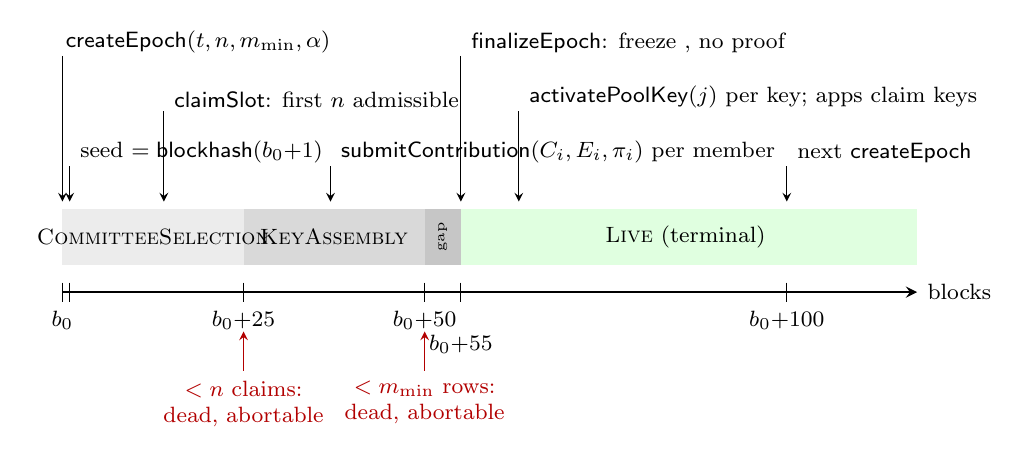
\begin{tikzpicture}[x=0.092cm, y=1cm, font=\footnotesize, >=stealth]
  % block axis
  \draw[->, thick] (0,0) -- (118,0) node[right] {blocks};
  \foreach \x/\l in {0/$b_0$, 25/$b_0{+}25$, 50/$b_0{+}50$, 100/$b_0{+}100$} {
    \draw (\x,0.12) -- (\x,-0.12);
    \node[below] at (\x,-0.12) {\l};
  }
  \draw (1,0.12) -- (1,-0.12); \draw (55,0.12) -- (55,-0.12);
  \node[below] at (55,-0.42) {$b_0{+}55$};
  % phases
  \fill[gray!15] (0,0.35) rectangle (25,1.05);
  \fill[gray!30] (25,0.35) rectangle (50,1.05);
  \fill[gray!45] (50,0.35) rectangle (55,1.05);
  \fill[green!12] (55,0.35) rectangle (118,1.05);
  \node at (12.5,0.7) {\textsc{CommitteeSelection}};
  \node at (37.5,0.7) {\textsc{KeyAssembly}};
  \node[rotate=90, font=\tiny] at (52.5,0.7) {gap};
  \node at (86,0.7) {\textsc{Live} (terminal)};
  % events above, three label rows
  \draw[->] (0,3.0) -- (0,1.15);
  \node[anchor=south west, align=left, inner sep=1pt] at (0,3.0) {$\mathsf{createEpoch}(t,n,m_{\min},\alpha)$};
  \draw[->] (1,1.6) -- (1,1.15);
  \node[anchor=south west, inner sep=1pt] at (2,1.6) {seed $= \mathsf{blockhash}(b_0{+}1)$};
  \draw[->] (14,2.3) -- (14,1.15);
  \node[anchor=south west, inner sep=1pt] at (15,2.3) {$\mathsf{claimSlot}$: first $n$ admissible};
  \draw[->] (37,1.6) -- (37,1.15);
  \node[anchor=south west, inner sep=1pt] at (38,1.6) {$\mathsf{submitContribution}(\vct{C}_i, \vct{E}_i, \pi_i)$ per member};
  \draw[->] (55,3.0) -- (55,1.15);
  \node[anchor=south west, inner sep=1pt] at (56,3.0) {$\mathsf{finalizeEpoch}$: freeze $\QUAL$, no proof};
  \draw[->] (63,2.3) -- (63,1.15);
  \node[anchor=south west, inner sep=1pt] at (64,2.3) {$\mathsf{activatePoolKey}(j)$ per key; apps claim keys};
  \draw[->] (100,1.6) -- (100,1.15);
  \node[anchor=south west, inner sep=1pt] at (101,1.6) {next $\mathsf{createEpoch}$};
  % abort arrows below
  \draw[->, red!70!black] (25,-1.0) -- (25,-0.5);
  \node[below, red!70!black, align=center] at (25,-1.0) {$< n$ claims:\\dead, abortable};
  \draw[->, red!70!black] (50,-1.0) -- (50,-0.5);
  \node[below, red!70!black, align=center] at (50,-1.0) {$< m_{\min}$ rows:\\dead, abortable};
\end{tikzpicture}
\caption{Epoch lifecycle on the block axis, with the deployment script's default windows. Finalization takes no proof and only freezes $\QUAL$; each of the $\Kmax$ pool keys is activated afterwards by its own proof, and an application claims the next activated key. An epoch that can still be finalized cannot be aborted; \textsc{Live} is terminal and overlaps with the next epoch's preparation, which may start ahead of cadence when the pool runs low.}
\label{fig:lifecycle}
\end{figure}
